% =========================================================================== %

\begin{frame}[t,plain]
\titlepage
\end{frame}

% =========================================================================== %

\begin{frame}[fragile]{Recap}
%
\begin{columns}[T]
\column{.5\linewidth}
\begin{itemize}
\item Kompilierzeit vs. Laufzeit
\item \texttt{malloc}, \texttt{calloc} und \texttt{free}
	\begin{itemize}
	\item Speicherplatz reservieren und Freigeben
	\item Zählung in Bytes bzw. Records
	\end{itemize}
\item Typenlose Pointer -- \mintinline{c}{void *}
\item \texttt{realloc}
	\begin{itemize}
	\item Größe eines bestehenden Arrays ändern
	\item Lässt Werte ggf. \enquote{umziehen}
	\end{itemize}
\end{itemize}
%
\column{.5\linewidth}
\begin{itemize}
\item Unterschiedliche Wirkung von \mintinline{c}{sizeof} auf automatische und dynamische Arrays
\item Möglichkeit mehrdimensionaler Arrays
\item Heap und Stack
\item \emph{Fragen}?
\end{itemize}
\end{columns}
%
\end{frame}

% =========================================================================== %

\begin{frame}{Script}
%
\begin{itemize}
\item Kapitel 10
	\begin{itemize}
	\item 10.1. Sammlungen von Werten: \mintinline{c}{struct}s
	\item 10.2. Casting-Interface: \mintinline{c}{union}s
	\item 10.3. Automatisch numerierte Symbole: \mintinline{c}{enum}s
	\end{itemize}
\end{itemize}
%
\end{frame}

% =========================================================================== %

\begin{frame}{\inC{struct}s -- Motivation}
%
\begin{itemize}
\item Aufgabe: Mehrere zusammenhängende Datensätze
\item Z.\,B.: Telefonbuch: Für jede Person
	\begin{itemize}
	\item Vorname
	\item Nachname
	\item Telefonnummer
	\item \ldots
	\end{itemize}
\item Bisher: Für jede Information eigene (Array-)Variable
\item Ziel: Eine (Array-)Variable, die alle diese Informationen aufnimmt
\item[\Thus] neuer Datentyp
\end{itemize}
%
\end{frame}

% =========================================================================== %

\begin{frame}[fragile]{\inC{struct}s -- \enquote{Container-Datentypen}}
%
\vspace{-10pt}
\begin{columns}[b]
\column{.5\linewidth}
%\begin{Large}
%\inC{struct}s -- \enquote{Container-Datentypen}
%\vspace{-5pt}
%\end{Large}
%
\small
\begin{itemize}
\item Definiert neuen Datentyp (wie \mintinline{c}{int})
\item Vorstellung: \emph{Tabellenkopf} -- enthält noch nicht die Information selbst!
	\begin{itemize}
	\item \enquote{\mintinline{c}{int}} enthält auch noch keine Zahl, sondern nur \emph{Art der
		Information}
	\item erst eine \emph{Variable} vom Typ \mintinline{c}{int} speichert tatsächlich die Zahl
	\item Sprechweise: Eine \emph{Instanz des Datentyps}
	\end{itemize}
\item \texttt{struct} muss \emph{vor Verwendung} definiert sein
\end{itemize}
\begin{hintbox}
\footnotesize Objekte, die \enquote{in einem Gedanken} greifbar sind, zu einer \texttt{struct} zusammenfassen
\end{hintbox}
%
\column{.5\linewidth}
\begin{codebox}[Syntax -- Datentyp definieren]
\begin{minted}[fontsize=\footnotesize]{c}
struct Typenname {
   Datentyp Attribut1;
   Datentyp Attribut2;
   ...
};
\end{minted}
\end{codebox}
%
\begin{codebox}[Syntax -- Variable anlegen]
\begin{minted}[fontsize=\footnotesize]{c}
struct Typenname Variable;
\end{minted}
\end{codebox}
%
\begin{codebox}[Syntax -- Zugriff auf Element]
\begin{minted}[fontsize=\footnotesize]{c}
Variable.Attribut = Ausdruck;
\end{minted}
\end{codebox}
\end{columns}
%

\end{frame}

% =========================================================================== %

\begin{frame}[fragile]
%
\begin{codebox}[
	Beispiel: Deklaration einer \texttt{struct}, 
	on line,
	width=.46\linewidth,
	equal height group=visTablehead
]
\begin{minted}[linenos, fontsize=\scriptsize]{c}
struct Karteieintrag {
  char vorname[50];
  char nachname[50];
  int  geburtsjahr;
  int  geburtsmonat;
  int  geburtstag;
};

int main () {
   struct Karteieintrag Cessi, Chami;
   
   Cessi.geburtsjahr = 1897;
   Chami.geburtsjahr = 1996;
   
   strcpy(Chami.vorname, "Lisl");
   // ...
}
\end{minted}
\end{codebox}
%
\begin{tcolorbox}[
	title=Visualisierung: Sammlung Tabellenköfpe, 
	on line, 
	width=.53\linewidth,
	equal height group=visTablehead
]
\scriptsize
\begin{tabular}{|l|l|l|}
\toprule[1pt]
\emph{Tabellenkopf}		& \texttt{Cessi}	& \texttt{Chami}	\tabcrlf
\texttt{vorname}			& Ce				& Lisl			\tabcrlf
\texttt{nachname}		& Saurus 		& Kohlenstoff	\tabcrlf
\texttt{geburtsjahr}		& 1897			& 1996			\tabcrlf
\texttt{geburtsmonat}	& 9				& 9				\tabcrlf
\texttt{geburtstag}		& 30				& 26				\\
\bottomrule[1pt]
\end{tabular}
\vfill
\end{tcolorbox}
%
\end{frame}

% =========================================================================== %

\begin{frame}[fragile]{Erlaubte Operationen}
%
\texttt{struct}s stellen sehr vielfältige Ideen dar. Telefonbucheinträge, komplexe Zahlen, Spielkarten, ... sind allesamt sinnvoll in \texttt{struct}s abbildbar.

\vspace{3pt}
Folge dessen ist, dass die meisten Rechenoperationen nicht allgemeingültig erklärt werden können. Daher sind nur die Wertzuweisung (\texttt{=}) und der direkte Vergleich (\texttt{==} und \texttt{!=}) definiert.

\begin{tcbraster}[raster columns=2,
                  raster equal height,
                  nobeforeafter
                 ]
\begin{codebox}[Wertzuweisung]
\begin{minted}[fontsize=\scriptsize]{c}
struct sometype x, y;

x = y;
\end{minted}
\end{codebox}
%
\begin{codebox}[Vergleich]
\begin{minted}[fontsize=\scriptsize]{c}
if (x == y) {
  printf("Instanzen identisch.\n");
}
\end{minted}
\end{codebox}
\end{tcbraster}

Addition, Subtraktion, ... und Ordnung (\texttt{<}, \texttt{>}, ...), etc. dagegen sind nur indirekt über ihre Attribute möglich.
%
\end{frame}

% =========================================================================== %

\begin{frame}[fragile]
%
\tcbset{width=.495\linewidth, on line}
%
\begin{codebox}[Komplexe Zahlen]
\begin{minted}[fontsize=\scriptsize,linenos]{c}
#include <stdio.h>

struct complex {
  double real;
  double imag;
};

struct complex addComplex(
  struct complex z1, 
  struct complex z2
) {
  struct complex reVal = z1;
  reVal.real += z2.real;
  reVal.imag += z2.imag;
  return reVal;
}

\end{minted}
\end{codebox}
%
\begin{codebox}[... Fortsetzung]
\begin{minted}[fontsize=\scriptsize,linenos,firstnumber=last]{c}
int main (void) {
  struct complex com1, com2, com3;
  
  com1.real = 3;
  com1.imag = 4;
  
  com2.real = 5;
  com2.imag = 6;
  
  com3 = addComplex(com1, com2);
  
  printf("%lf %+lfi\n", 
    com3.real, 
    com3.imag
  );
}
\end{minted}
\end{codebox}
%
\end{frame}

% =========================================================================== %

\begin{frame}[fragile]{\mintinline{c}{typedef} -- Abkürzung für häufige Datentypen}
%
\begin{columns}[T]
\column{.4\linewidth}
\begin{itemize}
\item Legt Bezeichnung an, die ab sofort für einen Datentyp steht
\item Datentyp: belieg komplexer Ausdruck
\item Auch Modifier erlaubt
	\begin{itemize}
	\item Pointer-Symbol \texttt{*}
	\item \mintinline{c}{unsigned}
	\item Weitere Modifier: Siehe \href{http://en.cppreference.com/w/c/language/declarations}{cppreference.com}
	\end{itemize}
\item mehrere Definitionen mit einem Aufruf: Komma-Syntax (siehe Beispiel)
\end{itemize}
%
\column{.6\linewidth}
\begin{codebox}[Syntax -- Alias definieren]
\begin{minted}[fontsize=\footnotesize]{c}
typedef Datentyp Alias;
\end{minted}
\end{codebox}
%
\begin{codebox}[Syntax -- Variable über Alias anlegen]
\begin{minted}[fontsize=\footnotesize]{c}
Alias Variable;
\end{minted}
\end{codebox}
%
\begin{codebox}[Beispiel]
\begin{minted}[fontsize=\footnotesize]{c}
typedef unsigned long long big_t, * big_p;
big_t myVar;
big_p myVarPointer = &myVar;
\end{minted}
\end{codebox}
%
\end{columns}
%
\end{frame}

% =========================================================================== %

\begin{frame}[fragile]
%
\tcbset{width=.495\linewidth, height=6.8cm, on line}
%
\begin{codebox}[Komplexe Zahlen -- mit \texttt{typedef}]
\begin{minted}[fontsize=\scriptsize,linenos]{c}
#include <stdio.h>

struct _complex {
  double real;
  double imag;
};
typedef struct _complex complex;

complex addComplex(
  complex z1, 
  complex z2
) {
  complex reVal = z1;
  reVal.real += z2.real;
  reVal.imag += z2.imag;
  return reVal;
}

\end{minted}
\end{codebox}
%
\begin{codebox}[... Fortsetzung]
\begin{minted}[fontsize=\scriptsize,linenos,firstnumber=last]{c}
int main (void) {
  complex com1, com2, com3;
  
  com1.real = 3;
  com1.imag = 4;
  
  com2.real = 5;
  com2.imag = 6;
  
  com3 = addComplex(com1, com2);
  
  printf("%lf %+lfi\n", 
    com3.real, 
    com3.imag
  );
}
\end{minted}
\end{codebox}
%
\end{frame}

% =========================================================================== %

\begin{frame}[fragile]{Anonyme Typen}
%
\begin{columns}[T]
\column{.4\linewidth}
\begin{itemize}
\item Weitere Kontraktion/Abkürzung
\item \texttt{struct} erhält keinen eigenen Namen
\item Stattdessen: Beschreibung der \texttt{struct} direkt an den Alias gebunden
\item Verschachtelung möglich: \texttt{struct} als record einer anderen \texttt{struct}.
\end{itemize}
%
\column{.55\linewidth}
\vspace{-10pt}
\begin{codebox}[Beispiel -- Komplexe Zahlen]
\begin{minted}[fontsize=\footnotesize, linenos]{c}
/* Original-Code aus meiner
 * Bachelor-Arbeit */
 
typedef struct {
	double real;
	double imag;
} complex, * complex_p;

typedef struct {
	int       rows;
	int       cols;
	complex_p data;
} matrix, * matrix_p;
\end{minted}
\end{codebox}
%
\end{columns}
%
\end{frame}

% =========================================================================== %

\begin{frame}[fragile]{Recap bis hierhin}
%
\begin{itemize}
\item \inC{struct}s sind wie Formulare, in die mehrere \emph{unterschiedliche} Wertetypen eingetragen werden
\item In der Deklaration eines \inC{struct}s nennen wir die Datentypen, also die Felder unseres \enquote{Formulars}
\item Die einzelnen Elemente (\enquote{Bausteine}) einer \inC{struct} heißen \emph{Attribute}, \emph{Felder} oder \emph{Records}
\item Wir brauchen \emph{Instanzen} von \inC{struct}s, um sinnvoll damit zu arbeiten
\item Eine \inC{struct}-Instanz zusammen mit einem Attribut verhält sich wie eine \emph{einfache Variable}
\item Eine \inC{struct}-Instanz alleine beschreibt \emph{alle} Werte (\enquote{ein gesamtes, ausgefülltes Formular})
\item \inC{struct}s werden i.\;d.\;R. \emph{global} definiert (Datentyp im gesamten Programm relevant). Die \emph{Instanzen} sind selbstverständlich trotzdem \emph{lokal}.
\end{itemize}
%
\end{frame}

% =========================================================================== %

\begin{frame}[fragile]{\texttt{struct}s und Pointer (I)}
%
\begin{tcbraster}[raster columns=2,
                  raster equal height,
                  nobeforeafter
                 ]
\begin{tcolorbox}[title=Records mit Array-Type]
\small
Die Attribute eines \texttt{struct}s können selbst Pointer sein.\\
\Thus Bekannte Syntax-Elemente
\begin{itemize}
\item Dereferenzierung: \newline
	\texttt{*var.record}
\item Index-Zugriff: \newline
	\texttt{var.record[index]}
\item Adresse finden: \newline
	\texttt{\&var.record}
\item[$\Rightarrow$] Wie bei gewöhnlichen Arrays
\end{itemize}
\end{tcolorbox}
%
\begin{codebox}[Code]
\begin{minted}[fontsize=\scriptsize, linenos]{c}
typedef struct {
    double position[3];
    double momentum[3];
    double mass;
} motiondata, * motiondata_p;

int main () {
  motiondata obj;
  obj.position[0] = 7.4;

  scanf("%lf", &obj.mass);

  printf("%p\n" ,  obj.position   );
  printf("%lf\n", *obj.position   );
  printf("%lf\n",  obj.position[0]);
  printf("%lf\n",  obj.mass       );
\end{minted}
\end{codebox}
\end{tcbraster}
%
\end{frame}

% =========================================================================== %

\begin{frame}[fragile]{\texttt{struct}s und Pointer (II)}
%
\vspace{-5pt}
\begin{tcbraster}[raster columns=2,
                  raster equal height,
                  nobeforeafter
                 ]
\begin{tcolorbox}[title=Arrays von \texttt{struct}-Instanzen]
\small
Pointer auf \inC{struct}-Instanzen möglich:
\begin{itemize}
\item Dereferenzierung: 
	\tabto{3cm}
	\texttt{*var}
\item Index-Zugriff: 
	\tabto{3cm}
	\texttt{var[index]}
\item Adresse finden: 
	\tabto{3cm}
	\texttt{\&var}
\end{itemize}
Neue Syntax: Von Pointer zu Record
\begin{itemize}
\item \texttt{var\_p->record} \\
	gleichbedeutend zu \\
	\texttt{(*var\_p).record}
\item Auflösung \enquote{von rechts nach links}
\item Klammern werden beachtet
\end{itemize}
\end{tcolorbox}
%
\begin{codebox}[Code]
\begin{minted}[fontsize=\scriptsize, linenos, firstnumber=last]{c}
  motiondata   swarm[100];
  motiondata_p swarmEl = &swarm[1];

  swarm[0] = obj;
  swarm[1].position[0] = 2;
  swarmEl->mass = 7;

  printf("%lf\n", swarm[1].mass);
  printf("%lf\n", swarmEl->position[0]);

  // just to confuse you ;)
  *((*swarmEl).position) = 
     *(swarm[0].position);

  printf("%lf\n", swarmEl->position[0]);
}
\end{minted}
\end{codebox}
\end{tcbraster}
%
\end{frame}

% =========================================================================== %

\begin{frame}[fragile]
%
\begin{tcbraster}[raster columns=2,
                  raster equal height,
                  nobeforeafter
                 ]
\begin{codebox}[\texttt{struct}s in Funktionen]
\begin{minted}[fontsize=\scriptsize, linenos]{c}
#include <stdio.h>
#include <string.h>

typedef struct {
  char   firstName [20];
  char   lastName  [20];
  char   department[20];
  double salary;
} employee_t;

void printEmployee(employee_t employee) {
  printf("%20s | %20s | %20s | %8.2lf\n",
    employee.firstName,
    employee.lastName,
    employee.department,
    employee.salary
  );
}
\end{minted}
\end{codebox}
%
\begin{codebox}[...Fortsetzung]
\begin{minted}[fontsize=\scriptsize, linenos, firstnumber=last]{c}
int () {
  employee_t emps[2];
  
  strcpy(emps[0].firstName , "Vanessa");
  strcpy(emps[0].lastName  , "Raupe");
  strcpy(emps[0].department, "HR");
  emps       [0].salary    = 7000.00;
  
  strcpy(emps[1].firstName , "Rebecka");
  strcpy(emps[1].lastName  , "Rein");
  strcpy(emps[1].department, "R&D");
  emps       [1].salary    = 420.69;
  
  printEmployee(emps[0]);
  printEmployee(emps[1]);
}
\end{minted}
\end{codebox}
\end{tcbraster}
%
\end{frame}

% =========================================================================== %

\begin{frame}[fragile]
%
\tcbset{width=.55\linewidth, on line}
%
\begin{codebox}[\texttt{structs} in Funktionen, equal height group=GStrPtrXmp2]
\begin{minted}[fontsize=\scriptsize, linenos]{c}
#include <stdio.h>
#include <string.h>

typedef struct {
  char   firstName [20];
  char   lastName  [20];
  char   department[20];
  double salary;
} employee_t;

void printEmployee(employee_t * employee) {
  printf("%20s | %20s | %20s | %8.2lf\n",
    employee->firstName,
    employee->lastName,
    employee->department,
    employee->salary
  );
}
\end{minted}
\end{codebox}
%
\tcbset{width=.43\linewidth, on line}
%
\begin{hintbox}[Optimierung, equal height group=GStrPtrXmp2]
\small
\begin{itemize}
\item Funktionsaufruf: Parameter wird kopiert
\item Hier: 68 Bytes
\item Wiederholte Aufrufe: Spürbarer Aufwand
\item Alternativ: Nur Pointer übergeben
\item[$\Rightarrow$] nur 8 Bytes kopiert
\item Anpassungen in der Funktion (Signatur, Zugriff Attribute)
\item Anpassung im Aufruf: \mintinline{c}{printEmployee(&emps[i]);}
\end{itemize}
\end{hintbox}
%
\end{frame}

% =========================================================================== %

\begin{frame}[t,fragile]{\inC{struct}s und Scopes}
%
\vspace{-10pt}
\begin{columns}[T]
\column{.4\linewidth}
%
\begin{itemize}
\item Selbe Regeln wie für Variablen
\item Von außen nach innen
\item Keine \enquote{horizontale Sichtbarkeit} (getrennte Scopes auf selber Hierarchieebene
\end{itemize}
%
\begin{hintbox}
\texttt{struct}s und \texttt{enum}s werden \idR im gesamten Programm gebraucht -- global definieren
\end{hintbox}
%
\column{.55\linewidth}
\vspace{-10pt}
\begin{codebox}
\begin{minted}[fontsize=\scriptsize, linenos]{c}
typedef struct {int dummy;} tglobal;
void proc (void) {
    typedef struct {int dummy;} tproc;
//  tmain y;  -- no horizontal visibility
    tproc z;
}
int main (void) {
    typedef struct {int dummy;} tmain;
    tglobal x;
    tmain   y;
//  tproc   z; -- no horizontal visibility
    {
        typedef struct {int dummy;} tsub;
        tglobal a; tmain b; tsub c;
    }
//  tsub z;  -- no insight into scope
}
\end{minted}
\end{codebox}
\end{columns}

%
\end{frame}

% =========================================================================== %

\begin{frame}[fragile]{Initializer-Syntax}
%
\vspace{-10pt}
\begin{codebox}[Beispiel: Initializer-Syntax bei \texttt{struct}s]
\begin{minted}[linenos, fontsize=\scriptsize]{c}
typedef struct {
  int  jahr;
  int  monat;
  int  tag;
} Datum;

int main () {
  Datum tag = {1989, 3, 29};
  // tag = {1989, 3, 29}; -- Verboten
}
\end{minted}
\end{codebox}
%
\begin{itemize}
\item Weist Werte in Reihenfolge der Deklaration zu
	\begin{itemize}
	\item \texttt{jahr} $\leftarrow$ \texttt{1989}, \texttt{monat} $\leftarrow$ \texttt{3}, ...
	\end{itemize}
\item \emph{Ausschließlich} bei der Deklaration der Instanz möglich
\item Funktioniert hier dafür auch mit Strings
\end{itemize}
%
\end{frame}

% =========================================================================== %

\begin{frame}[fragile]
%
\tcbset{width=.6\linewidth, on line}
%
\begin{codebox}[Beispiel: Initializer-Syntax bei Strings]
\begin{minted}[linenos, fontsize=\scriptsize]{c}
#include <stdio.h>
#include <stdlib.h>

typedef struct {
  char   constSizeArray[50];
  char * charPointer;
} twoStrings;

int main () {
  twoStrings x = {"kleiner Biber",
                  "kleiner Biber"};
  
  printf("Startadresse der Instanz:\n"
         "\t%p\n",  (void *)(&x));
  printf("Adresse von constSizeArray:\n"
         "\t%p\n",  (void *)(x.constSizeArray));
  printf("Adresse von charPointer:\n"
         "\t%p\n",  (void *)(x.charPointer));
}
\end{minted}
\end{codebox}
%
\tcbset{width=.38\linewidth, on line}
%
\begin{cmdbox}[Ausgabe]
\begin{minted}[fontsize=\scriptsize]{text}
Startadresse der Instanz:
        0x7ffc0d4172c0
Adresse von constSizeArray:
        0x7ffc0d4172c0
Adresse von charPointer:
        0x562bd763b808
\end{minted}
\end{cmdbox}
%
\end{frame}

% =========================================================================== %

\begin{frame}[fragile]{\mintinline{c}{enum}s -- automatisch nummerierte Symbole}
%
\begin{columns}[T]
\column{.5\linewidth}
\vspace{-5pt}
\begin{itemize}
\item Definition von Konstanten mit aufsteigenden Werten
\item Gleichzeitig Definition von Alias für \mintinline{c}{int}
\item Hilft für besser lesbaren Code
\item Häufig in ALL CAPS
\item Anonyme \inC{enum}s möglich
\end{itemize}
%
\begin{codebox}[Syntax]
\begin{minted}[fontsize=\footnotesize]{c}
enum Name {
  Symbol_1,
  Symbol_2,
  ...
};
\end{minted}
\end{codebox}
%
\column{.5\linewidth}
\vspace{-7pt}
\begin{codebox}[Beispiel]
\begin{minted}[fontsize=\scriptsize, linenos]{c}
enum Cardsuits {
  HEARTS,
  DIAMOND,
  CLUB,
  SPADES
};
typedef struct {
  Cardsuits suit;
  value     val;
} Card;
Card myCard;
...
if (myCard.suit == HEARTS) {
  // Trumpfkarte
  ...
}
\end{minted}
\end{codebox}
\end{columns}
%
\end{frame}

% =========================================================================== %

\begin{frame}[fragile]{\inC{union}s -- Typecasting-Interfaces}
%
\begin{itemize}
\item Ähnlich \mintinline{c}{struct}s
\item Alle Elemente beginnen an derselben Speicherstelle
\item Effektiv: Typecasting
\item Elektronik-Anwendungen
\end{itemize}

\tcbset{width=.35\linewidth, on line}
\begin{codebox}[Beispiel, equal height group = xmpUnion]
\begin{minted}[fontsize=\scriptsize, linenos]{c}
typedef union {
  int i;
  char c[4];
} intUnion;

int main () {
  intUnion u;
  u.i = 65535;
}
\end{minted}
\end{codebox}
%
\tcbset{width=.6\linewidth, on line}
\begin{tcolorbox}[title=Speicherbild, equal height group = xmpUnion]
\begin{center}
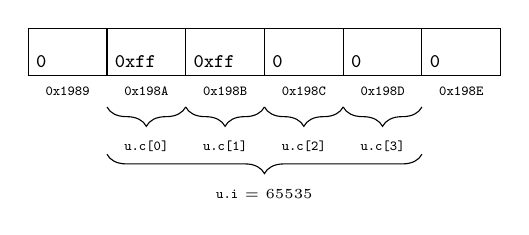
\begin{tikzpicture}
  [ 
    cell/.style={
       text width =8mm,
       text height=4mm, 
       draw=black, 
       inner sep  =1mm
    },
    ld/.style={
       draw=blue,
       shorten >=2pt,
       ->
    }
  ]
  \node (c00) at ( 0.0,1) [cell] {\ttfamily \scriptsize  0  };
  \node (c01) at ( 1.0,1) [cell] {\ttfamily \scriptsize 0xff};
  \node (c02) at ( 2.0,1) [cell] {\ttfamily \scriptsize 0xff};
  \node (c03) at ( 3.0,1) [cell] {\ttfamily \scriptsize  0  };
  \node (c04) at ( 4.0,1) [cell] {\ttfamily \scriptsize  0  };
  \node (c05) at ( 5.0,1) [cell] {\ttfamily \scriptsize  0  };

  \node (p00) at ( 0.0,0.5)      {\ttfamily \tiny 0x1989};
  \node (p01) at ( 1.0,0.5)      {\ttfamily \tiny 0x198A};
  \node (p02) at ( 2.0,0.5)      {\ttfamily \tiny 0x198B};
  \node (p03) at ( 3.0,0.5)      {\ttfamily \tiny 0x198C};
  \node (p04) at ( 4.0,0.5)      {\ttfamily \tiny 0x198D};
  \node (p05) at ( 5.0,0.5)      {\ttfamily \tiny 0x198E};
  
  \draw [decorate, decoration={brace,amplitude=7pt, mirror}, xshift=-0pt, yshift=0pt]
  		( 0.5, -0.3) -- ( 4.5, -0.3) node [midway, yshift=-0.5cm] 
		(braceArrayPreResize) {\tiny \texttt{u.i} = 65535};

  \draw [decorate, decoration={brace,amplitude=7pt, mirror}, xshift=-0pt, yshift=0pt]
  		( 0.5, 0.3) -- ( 1.5, 0.3) node [midway, yshift=-0.5cm] 
		(braceArrayPreResize) {\tiny \texttt{u.c[0]}};

  \draw [decorate, decoration={brace,amplitude=7pt, mirror}, xshift=-0pt, yshift=0pt]
  		( 1.5, 0.3) -- ( 2.5, 0.3) node [midway, yshift=-0.5cm] 
		(braceArrayPreResize) {\tiny \texttt{u.c[1]}};

  \draw [decorate, decoration={brace,amplitude=7pt, mirror}, xshift=-0pt, yshift=0pt]
  		( 2.5, 0.3) -- ( 3.5, 0.3) node [midway, yshift=-0.5cm] 
		(braceArrayPreResize) {\tiny \texttt{u.c[2]}};

  \draw [decorate, decoration={brace,amplitude=7pt, mirror}, xshift=-0pt, yshift=0pt]
  		( 3.5, 0.3) -- ( 4.5, 0.3) node [midway, yshift=-0.5cm] 
		(braceArrayPreResize) {\tiny \texttt{u.c[3]}};
\end{tikzpicture}
\end{center}
\end{tcolorbox}
%
\end{frame}